\documentclass[12pt,letterpaper]{article}
\usepackage{graphicx}

\usepackage[margin=1in]{geometry}

\begin{document}

\begin{flushright}
Homework 2: SSA, Constant Propagation, and Value Numbering\\
Paul Vines and Eric Mullen\\
CSE 501\\
\end{flushright}
\subsubsection*{Translation to SSA}
In order to transalte to SSA, we first calculate the dominance
frontier, using the method provided in the slides. We store the
frontier as a map from a basic block to a set of basic blocks. Next we
find all of the local variables defined in this particular method, and
use the standard phi insertion algorithm provided to insert phi nodes
at the beginning of basic blocks where needed. Finally, we call rename
on the root of the dominator tree, which goes through and converts all
instruction operands to their SSA forms. Note that the only
instruction that can store a new value in a local variable is the move
instruction, which coupled with phi nodes are the only two places
where a variable's SSA subscript will ever have to be
incremented. Finally, we insert our renamed arguments in the phi nodes
of our successors in the control flow graph, and recursively rename
all of our children in the dominator tree. The slides were very
confusing as to whether successors meant CFG or dominator successors,
as SUCC(X) meant both, depending on context. Finally, as we are liable
to move around basic blocks, we insert explicit branches at the end of
all basic blocks.

\subsubsection*{Constant Propagation}
Constant Propagation was performed on the SSA-form instructions by
adding a lattice-cell value to each instruction in a wrapper
expression class. Expressions are stored in a HashMap keyed by the
instruction number, except Move expressions, which are keyed by the
hashcode of the variable they are being stored in. When constructing
these expression objects the lattice value is assigned based on the
instruction type and operands: Arithmetic instructions, comparison,
moves, and stores, are initialized to Top unless all operands are
Const, then Const Phi instructions are assigned Top All other operands
are assigned Bottom, as they either do not have results that are in
scope of intraprocedural analysis or should not ever be used as an
operand (e.g. Write).

All expression that are constants are analyzed to determine their
constant value by inspecting their operands (Immediates at this point)
and performing the computation associated with their instruction and
storing the results in the expression object.

The SSA edges list is a HashMap of sets of expressions keyed by an
expression. It is constructed by iterating through all expressions,
for each operand in the expression, the set corresponding to that
operand is retrieved and the expression is added to the set,
indicating this expression is affected by the value of the expression
corresponding to its operand. O(n)

After expressions and the SSA Edges have been constructed, every SSA
Edge keyed to a non-Top variable is added to the worklist queue.
Until the worklist is not empty, an SSA Edge is dequeueued. The value
of the destination of the edge is reevaluated based on the source. If
the source is a Bottom, the destination becomes Bottom. If the source
is Const then, unless the destination is a Phi node or is Bottom, the
destination is set to Const. If the destination is a Phi then the
lattice value is reduced to Bottom unless all operands of the Phi node
are Const and have the same Const values. Because of this, all Phi
node evaluation is delayed until either all the Phi node arguments are
non-Top or only Phi nodes.  If an expression is made Const then its
value is determined based on the values of its operands.

After the worklist is empty all expressions will now have a non-Top
lattice value. All arithmetic expressions with Const operands have
their operand replaced with Immediates of the correct
value. Conditional branches with Const conditiona operands are
replaced with unconditional branches or nops.  After constant operands
have been replaced, all Const instructions can be removed, unless they
are used in a non-Const Phi node.

\subsubsection*{Value Numbering}

We implement a global (per method) value numbering scheme, described
in the dominator based value numbering technique in the paper by
Briggs, Cooper and Simpson. It is slightly different, in that it never
proves that a phi node is meaningless or redundant, and thus does not
remove them. Other than this small difference, it is functionally
equivalent to the literature.

The key to understanding our implementation of value numbering is to
realize that the name is simply an implementation detail, and we
decided to implement it a different way. In our scheme, a value number
is not, in fact, a number, but contains a reference to the previous
value (register or local) that holds the already computed value.

We keep three maps around to store available expressions. One is a map
from instruction operands to existing value numbers, so that we can
replace all operands on future instructions with their value numbered
counterparts. The other two maps are from binary expressions to value
numbers, and unary expressions to value numbers. We define a subset of
all operations that can actually be value numbered (arithmetic and the
like, as well as null checks and type checks), and insert any
instruction that uses that operation into our maps of available
expressions. If we come across an expression that we've already
calculated, we insert the register or local that was the result of
that expression into our available values map, and mark that
instruction as dead. When translating out of SSA, all instructions not
marked live are eliminated, though we do not do a full dead code
elimination pass. Finally, when value numbering is concluded, we
remove all the value numbers from the code.

\subsubsection*{Translation from SSA}

There are only a few concerns that we deal with when translating back
out of SSA. First, we remove phi functions, and replace them with
moves at the end of predecessor basic blocks. We don't manipulate the
control flow graph by adding new nodes, we simply add moves at the end
of existing blocks. We don't add a move if the source or dest value of
the move is already proven to be dead in a previous stage.

Next, we calculate how many local variables we have now, and fix up
the offsets for them, as well as the amount of stack allocation done
by enter instructions. We do nothing to try to coallesce the large
number of local variables we introduce, though we could use Chaitin's
heuristic to generate a fairly good coloring (just never spill), and
decrease the number of variables that way.

Finally, we renumber all of our instructions, and fix up the register
and location operands that now point to instructions with a different
number. This wouldn't be necessary except that the interpreter can
only take instructions in order, and thus we must renumber before
emitting.

\subsection*{Results}


\begin{center}
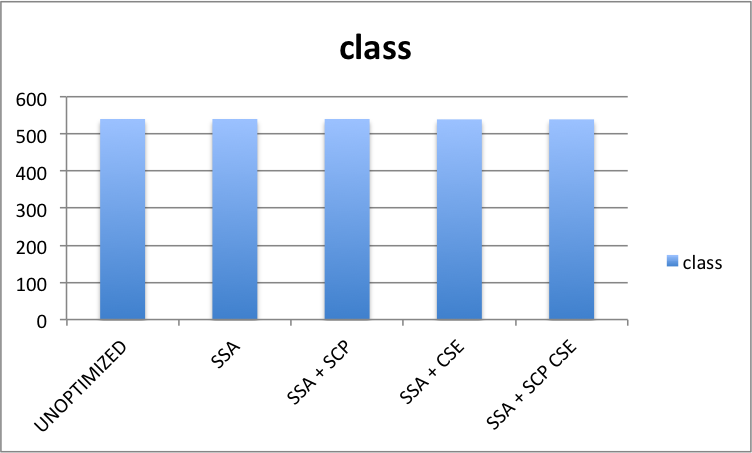
\includegraphics[width=4in]{/Users/plvines/Documents/Compilers/cse_501/hw2/writeup/class.png}
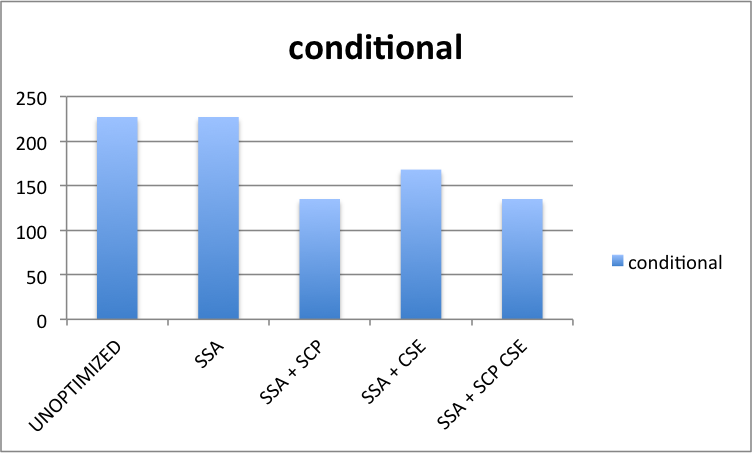
\includegraphics[width=4in]{/Users/plvines/Documents/Compilers/cse_501/hw2/writeup/conditional.png}
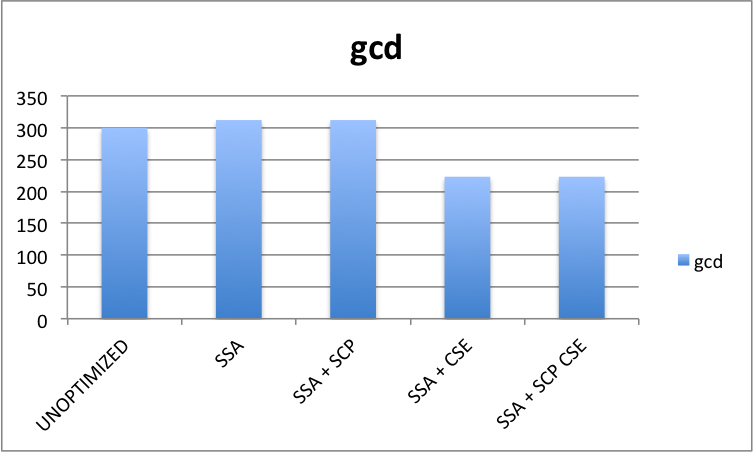
\includegraphics[width=4in]{/Users/plvines/Documents/Compilers/cse_501/hw2/writeup/gcd.png}
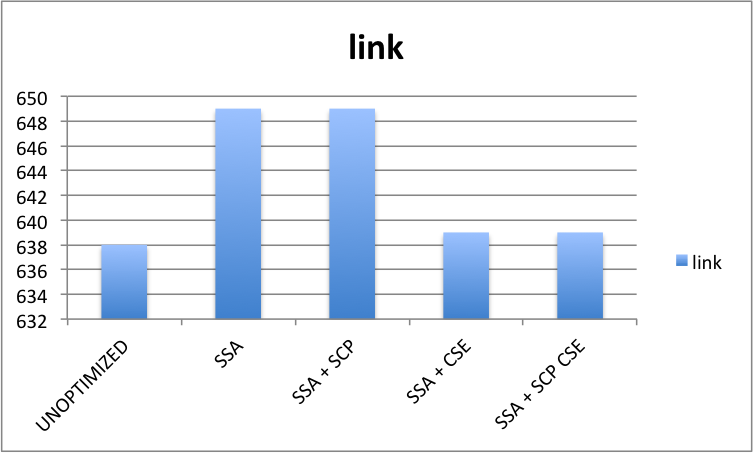
\includegraphics[width=4in]{/Users/plvines/Documents/Compilers/cse_501/hw2/writeup/link.png}
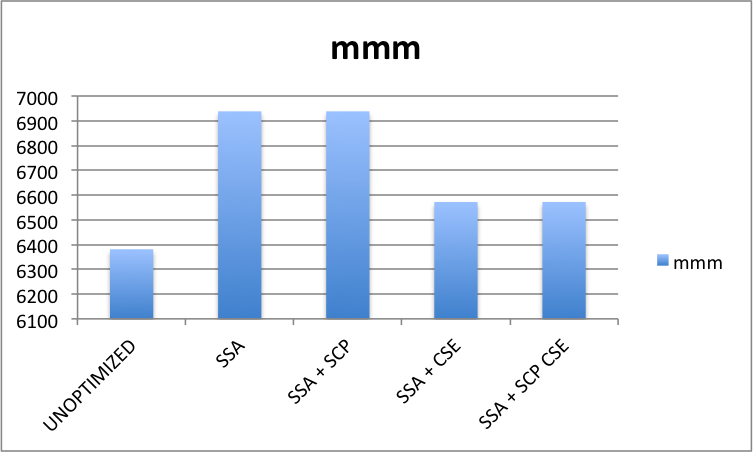
\includegraphics[width=4in]{/Users/plvines/Documents/Compilers/cse_501/hw2/writeup/mmm.png}
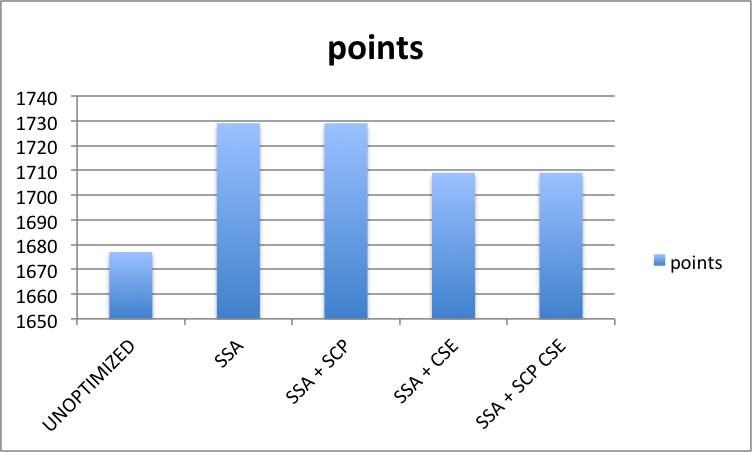
\includegraphics[width=4in]{/Users/plvines/Documents/Compilers/cse_501/hw2/writeup/points.png}
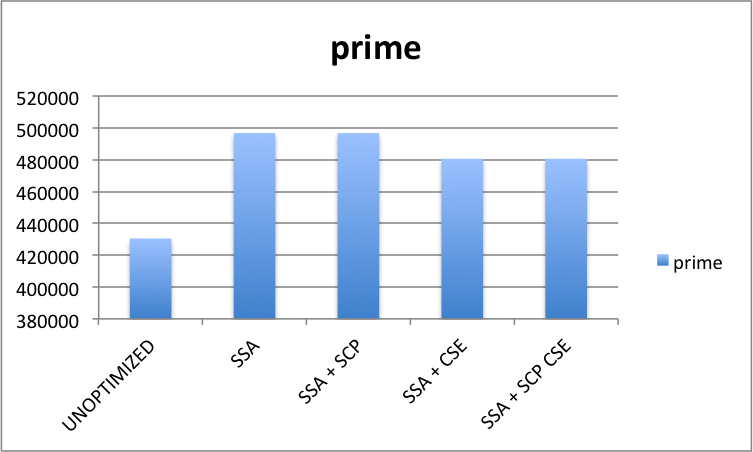
\includegraphics[width=4in]{/Users/plvines/Documents/Compilers/cse_501/hw2/writeup/prime.png}
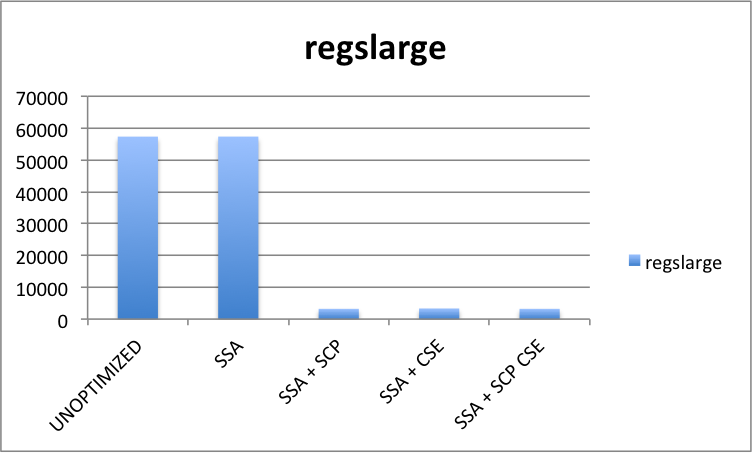
\includegraphics[width=4in]{/Users/plvines/Documents/Compilers/cse_501/hw2/writeup/regslarge.png}
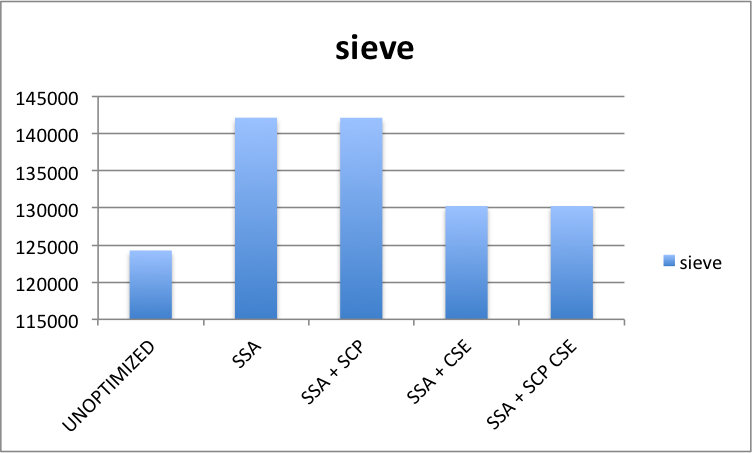
\includegraphics[width=4in]{/Users/plvines/Documents/Compilers/cse_501/hw2/writeup/sieve.png}
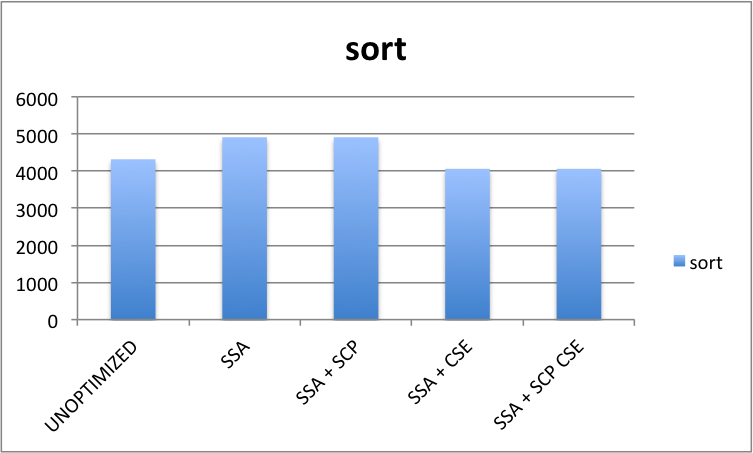
\includegraphics[width=4in]{/Users/plvines/Documents/Compilers/cse_501/hw2/writeup/sort.png}
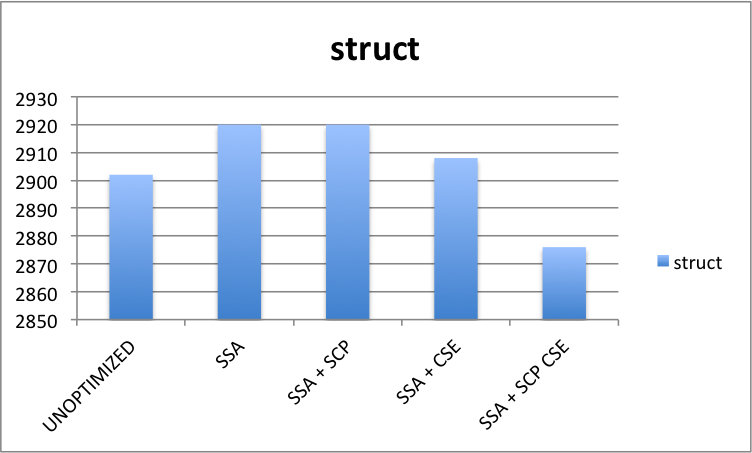
\includegraphics[width=4in]{/Users/plvines/Documents/Compilers/cse_501/hw2/writeup/struct.png}
\end{center}

\end{document}
